\section{Results}
\label{sec:results}

\subsection{Adversarial Robustness}

\Tabref{tab:adversarial} presents the main adversarial robustness results. All three thicket variants achieve PGD-20 accuracy within 0.2\% of the single model, providing no meaningful robustness improvement. At $\sigma = 0.001$ --- the largest viable perturbation scale --- ensemble members have a disagreement rate of only 0.6\%, meaning they are functionally identical. The white-box PGD attacker trivially finds adversarial examples that fool all members simultaneously.

\begin{table}[t]
    \centering
    \caption{Adversarial robustness comparison. Thicket ensembles ($\sigma = 0.001$, $K = 5$) provide no improvement over a single model, while adversarial training (\pgdat) achieves 78.5\% PGD accuracy. Best results in \textbf{bold}.}
    \begin{tabular}{@{}lccc@{}}
        \toprule
        Method & Clean Acc (\%) & PGD-20 Acc (\%) & FGSM Acc (\%) \\
        \midrule
        Single Model & 94.1 & 12.6 & 47.8 \\
        Gaussian \thicket & 94.0 & 12.5 & 47.4 \\
        Orthogonal \thicket & 94.0 & 12.4 & 47.2 \\
        Layer-Scaled \thicket & 94.1 & 12.6 & 47.8 \\
        \midrule
        \deepens (3 members) & \textbf{94.7} & 19.7 & 53.2 \\
        \pgdat & 91.2 & \textbf{78.5} & \textbf{79.7} \\
        \bottomrule
    \end{tabular}
    \label{tab:adversarial}
\end{table}

The deep ensemble achieves 19.7\% PGD accuracy --- a 56\% relative improvement over the single model --- demonstrating that genuine functional diversity from independent training trajectories does confer some robustness. However, this is still far from the 78.5\% achieved by adversarial training, confirming that diversity alone is insufficient for strong adversarial robustness.

\subsection{The Sensitivity Cliff}
\label{sec:sensitivity}

\Tabref{tab:sigma} reveals the fundamental constraint underlying our negative result. There is a sharp phase transition between $\sigma = 0.01$ (92.4\% accuracy, 9.1\% disagreement) and $\sigma = 0.02$ (28.4\% accuracy, 61.4\% disagreement). The model is catastrophically destroyed by perturbations of magnitude $\sim$0.02, which corresponds to roughly 2\% of parameter magnitudes. No intermediate regime exists where both high accuracy and meaningful diversity coexist.

\begin{table}[t]
    \centering
    \caption{Perturbation scale $\sigma$ controls a sharp tradeoff between accuracy and diversity. A phase transition between $\sigma = 0.01$ and $\sigma = 0.02$ leaves no regime where both high accuracy and high diversity coexist.}
    \begin{tabular}{@{}lccc@{}}
        \toprule
        $\sigma$ & Clean Acc (\%) & Mean Candidate Acc (\%) & Disagreement Rate \\
        \midrule
        0.001 & 94.0 & 94.1 & 0.006 \\
        0.005 & 93.8 & 93.6 & 0.033 \\
        0.01 & 92.4 & 89.9 & 0.091 \\
        0.02 & 28.4 & 14.0 & 0.614 \\
        0.05 & 11.7 & 10.2 & 0.830 \\
        \bottomrule
    \end{tabular}
    \label{tab:sigma}
\end{table}

\Figref{fig:sigma_sweep} visualizes this tradeoff, showing the cliff-like behavior rather than the gradual tradeoff one might expect. This contrasts sharply with LLMs, where \citet{gan2026neural} report that models with billions of parameters tolerate substantially larger perturbations.

\begin{figure}[t]
    \centering
    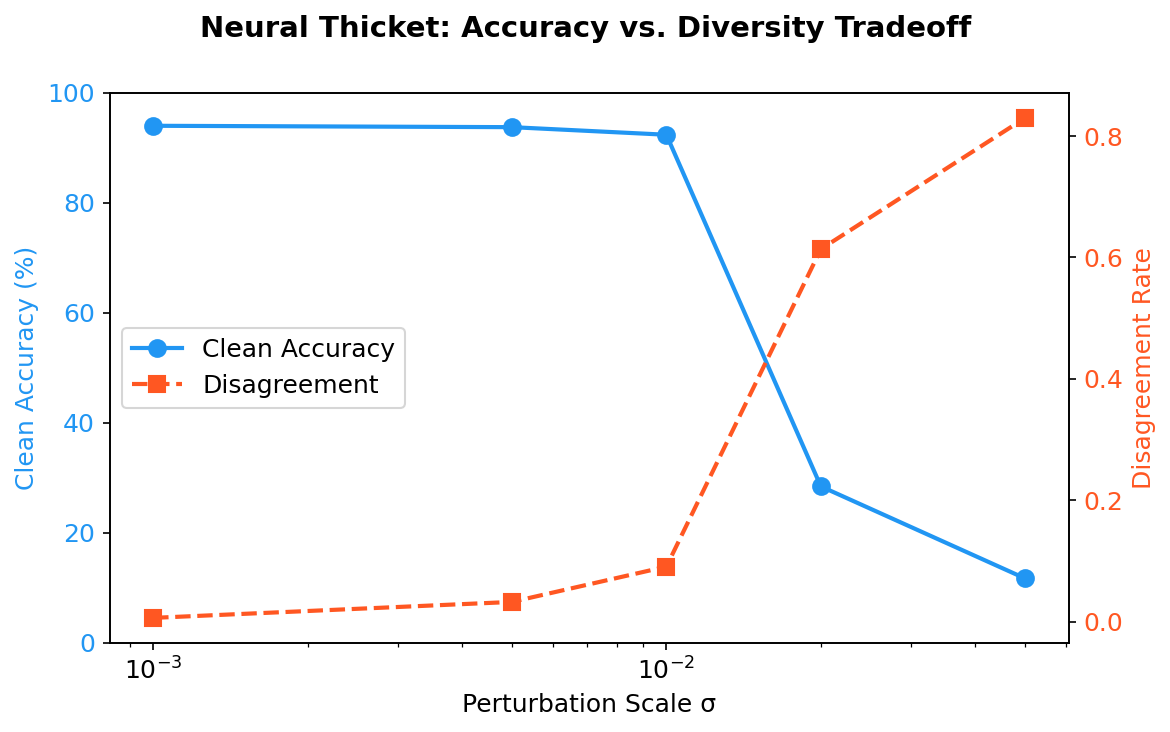
\includegraphics[width=0.95\linewidth]{figures/sigma_sweep.png}
    \caption{Accuracy vs.\ diversity across perturbation scales $\sigma$. A sharp phase transition occurs between $\sigma = 0.01$ and $\sigma = 0.02$: accuracy collapses from 92.4\% to 28.4\% while disagreement jumps from 9.1\% to 61.4\%. No useful intermediate regime exists.}
    \label{fig:sigma_sweep}
\end{figure}

\subsection{OOD Detection}

\Tabref{tab:ood} presents OOD detection results for \cifarten (in-distribution) vs.\ \svhn (OOD). All methods achieve similar AUROC ($\sim$0.93 with energy scores), with thicket ensembles performing comparably to the deep ensemble. The energy score consistently outperforms both MSP and mutual information across all ensemble methods.

\begin{table}[t]
    \centering
    \caption{OOD detection performance (\cifarten $\to$ \svhn). Energy scores outperform mutual information across all methods. Thicket ensembles perform comparably to the deep ensemble. Best results in \textbf{bold}; lower FPR@95 is better.}
    \begin{tabular}{@{}lcccc@{}}
        \toprule
        Method & MSP AUROC & Energy AUROC & MI AUROC & Energy FPR@95 \\
        \midrule
        Gaussian \thicket & 0.913 & 0.933 & 0.894 & 0.389 \\
        Orthogonal \thicket & 0.914 & 0.934 & \textbf{0.918} & 0.391 \\
        Layer-Scaled \thicket & 0.913 & 0.933 & 0.901 & 0.394 \\
        \midrule
        \deepens & \textbf{0.917} & \textbf{0.937} & 0.908 & \textbf{0.415} \\
        \bottomrule
    \end{tabular}
    \label{tab:ood}
\end{table}

Notably, the orthogonal thicket achieves MI AUROC of 0.918 compared to 0.894 for the Gaussian variant --- a meaningful improvement in the diversity-dependent metric, suggesting that orthogonal perturbations do create slightly more functional diversity. However, this advantage does not translate to adversarial robustness improvements.

\subsection{Ensemble Size Ablation}

\Tabref{tab:ablation} shows that increasing ensemble size $K$ from 3 to 10 has negligible effect on both clean and robust accuracy. Since all members at $\sigma = 0.001$ are near-clones (0.6\% disagreement), adding more identical copies cannot improve robustness.

\begin{table}[t]
    \centering
    \caption{Ensemble size ablation ($\sigma = 0.001$, Gaussian perturbation). Increasing $K$ has no effect because all members are near-identical at this perturbation scale.}
    \begin{tabular}{@{}lcc@{}}
        \toprule
        $K$ & Clean Acc (\%) & PGD-20 Acc (\%) \\
        \midrule
        3 & 94.0 & 12.5 \\
        5 & 94.1 & 12.4 \\
        10 & 94.0 & 12.4 \\
        \bottomrule
    \end{tabular}
    \label{tab:ablation}
\end{table}

\begin{figure}[t]
    \centering
    \begin{subfigure}[b]{0.48\textwidth}
        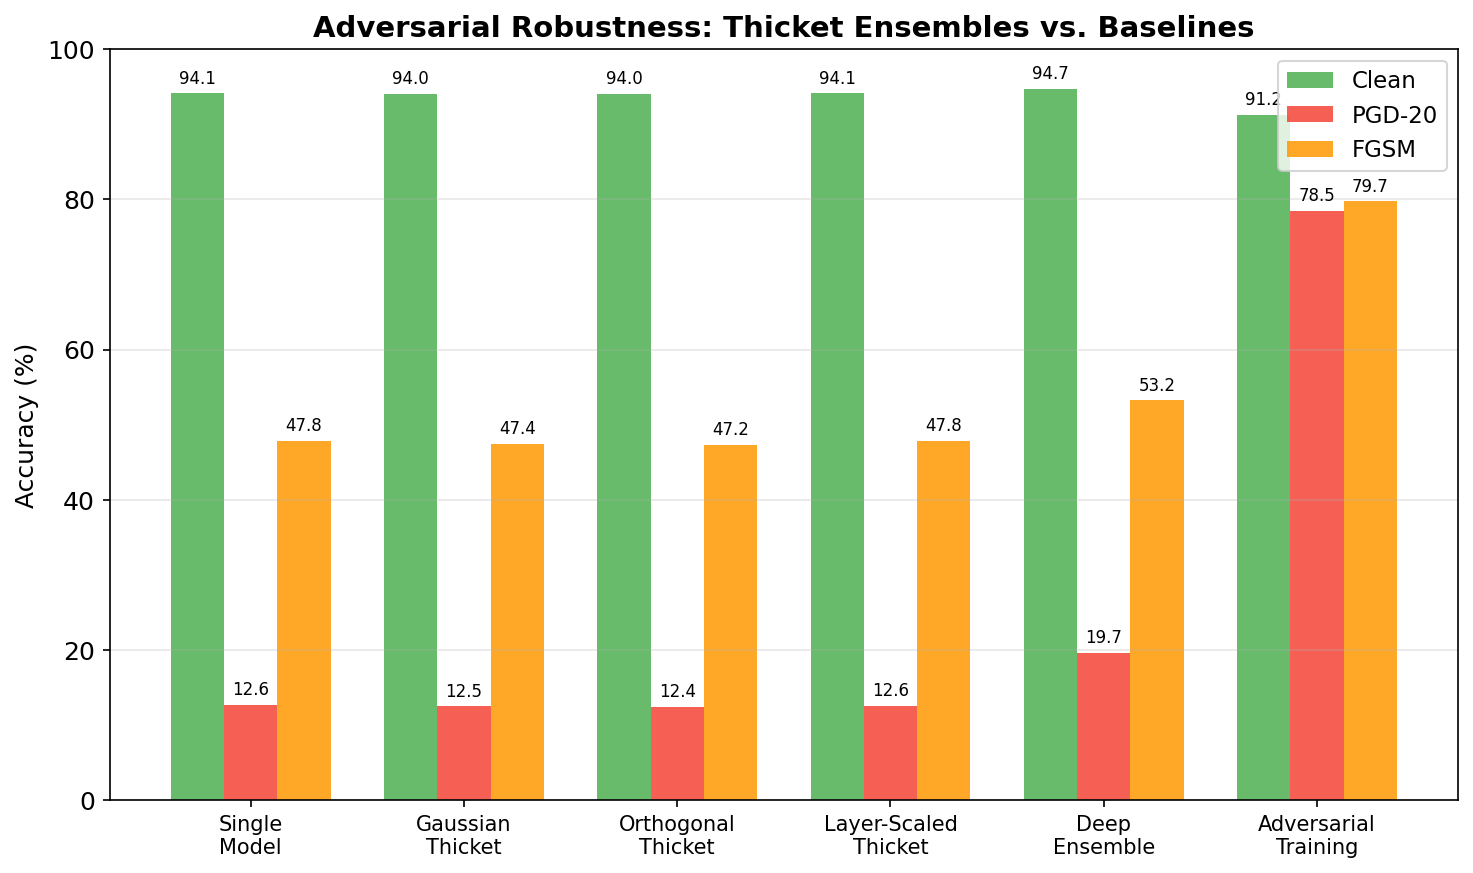
\includegraphics[width=\textwidth]{figures/adversarial_robustness.png}
        \caption{Adversarial robustness}
        \label{fig:adv_bar}
    \end{subfigure}
    \hfill
    \begin{subfigure}[b]{0.48\textwidth}
        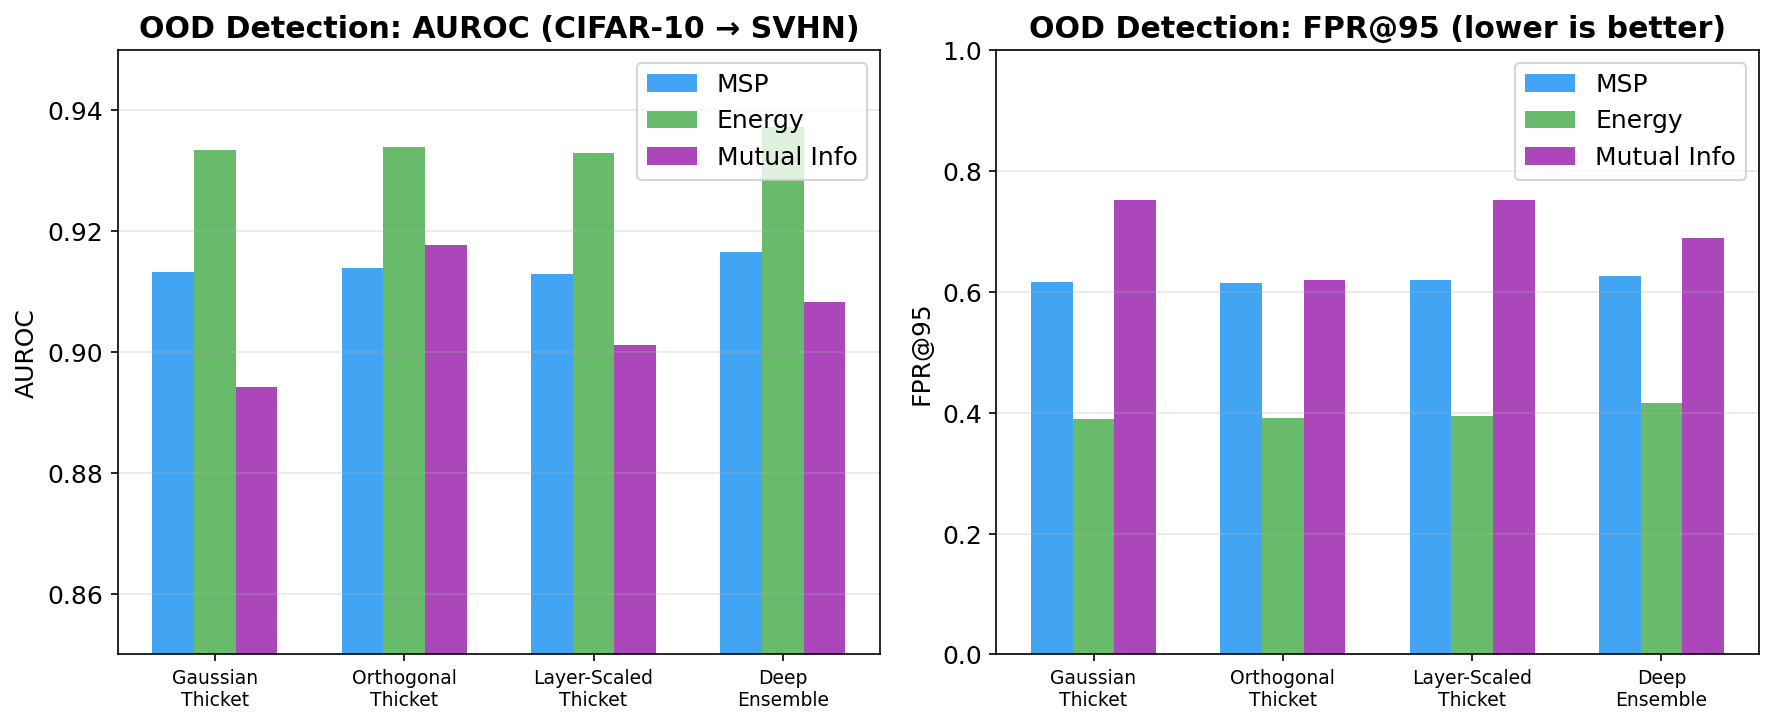
\includegraphics[width=\textwidth]{figures/ood_detection.png}
        \caption{OOD detection}
        \label{fig:ood_bar}
    \end{subfigure}
    \caption{\figleft Adversarial robustness: thicket ensembles match the single model under PGD-20 and FGSM; only adversarial training provides substantial robustness. \figright OOD detection: all ensemble methods achieve similar AUROC with energy scores.}
    \label{fig:main_results}
\end{figure}
